\begin{minipage}[t]{180mm}
\fcolorbox{black}{white}{
\begin{minipage}[b]{30mm}
\includegraphics[width=0.5\linewidth]{unflogo.pdf}
\end{minipage}
\begin{minipage}[b]{100mm}
\Huge \textbf{UNF NEWZ} \\
\Large -- jyder er også hvirveldyr!
\end{minipage}
\begin{minipage}[b]{50mm}
\Large Søndag 15.07.2013 \\
\normalsize Redigeret i \LaTeX\ af \\ SOM, MGS, KUM, TAL, JAM
\end{minipage}
}
\end{minipage}



\begin{minipage}[b]{0.95\linewidth}
\begin{minipage}[t]{0.47\textwidth}
\vspace{3mm}

\end{minipage}
\hfill\begin{minipage}[t]{0.47\textwidth}

\vspace{1mm}
\tikzstyle{mybox} = [draw=white, fill=blue!20, very thick,
    rectangle, rounded corners, inner sep=10pt, inner ysep=20pt]
\tikzstyle{fancytitle} =[fill=red, text=white]

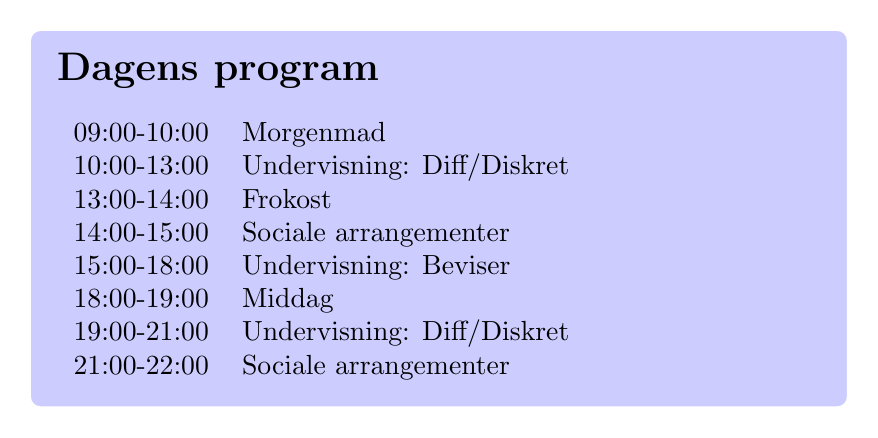
\begin{tikzpicture}
\node [mybox] (box){%
\begin{minipage}{0.80\textwidth}
\vspace{-4mm}\section*{Dagens program}
\begin{tabular}{ll}
09:00-10:00 & Morgenmad \\
10:00-13:00 & Undervisning: Diff/Diskret \\
13:00-14:00 & Frokost \\
14:00-15:00 & Sociale arrangementer \\
15:00-18:00 & Undervisning: Beviser \\
18:00-19:00 & Middag \\
19:00-21:00 & Undervisning: Diff/Diskret \\
21:00-22:00 & Sociale arrangementer
\end{tabular}
\vspace{-4mm}
\end{minipage}
};
\end{tikzpicture}%



\end{minipage}
\end{minipage}
